\documentclass{article}
\usepackage[a4paper,margin=1in]{geometry}

\title{Fast and accurate protein false discovery rates on human
proteome study scale with Percolator 3.0}

\author{Matthew The,\\
Science for Life Laboratory,\\
School of Biotechnology,\\
Royal Institute of Technology - KTH,\\
Box 1031, 17121 Solna,\\ Sweden
\and 
Michael J. MacCoss,\\
Department of Genome Sciences,\\
School of Medicine,\\
University of Washington,\\
Seattle, Washington 98195,\\ United States of America
\and 
William S. Noble,\\
Department of Genome Sciences,\\
School of Medicine,\\
University of Washington,\\
Seattle, Washington 98195,\\ United States of America
\and
Lukas K\"{a}ll\\
Science for Life Laboratory,\\ School of Biotechnology,\\
Royal Institute of Technology - KTH\\ 
Box 1031, 17121 Solna,\\ Sweden}

\usepackage{setspace}
\usepackage{amsmath}
\usepackage{url}
%\usepackage{bbm}
\usepackage{dsfont} % preferrred over bbm in submission system
\usepackage{graphicx}
\usepackage[outdir=./img/]{epstopdf}
\usepackage{epsfig}

\begin{document}

\maketitle

\doublespacing

Keywords: mass spectrometry - LC-MS/MS, statistical analysis, 
data processing and analysis, protein inference, simulation


\newpage

\begin{abstract} 

Percolator is a popular tool to increase yield in shotgun proteomics
experiments and to assign reliable statistics, such as $q$~values and
posterior error probabilities, to peptides and peptide spectrum
matches (PSMs) from such experiments. Percolator's processing speed
has been sufficient for typical data sets with hundreds of thousands
of PSMs. With our new scalable approach, we can now also analyze
millions of PSMs in a matter of minutes on a commodity computer.
Furthermore, with the increasing awareness for the need for reliable
statistics on the protein level, we compared several
easy-to-understand protein inference methods and implemented the best
method in the Percolator package. We used Percolator 3.0 to analyze
the data from a recent study of the draft human proteome containing 20
million spectra (PM:24870542).

The source code and Ubuntu, Windows, MacOS and Fedora binary packages
are available from \url{https://github.com/percolator/percolator},
under Apache 2.0 license.
\end{abstract}

\newpage

\section*{Introduction}

Percolator~\cite{kall2007} has played a prominent part in the analysis
pipelines of shotgun proteomics experiments for the last decade, as a
post-processor of the results from database search engines such as
SEQUEST~\cite{eng1994}, MASCOT~\cite{cottrell1999},
X!Tandem~\cite{craig2004tandem} and MS-GF+~\cite{kim2008}. Not only
does Percolator give a significant boost in the number of significant
peptide spectrum matches (PSMs) or peptides, it also provides a
consistent statistical framework in which to interpret the search
results. As Percolator's running time is usually much lower than that
of the search engine, applying it as a post-processing step should be
the default choice when processing shotgun proteomics data. As part of
the continuous development and support of the Percolator package, we
present two major additions aimed at supporting analysis of studies on
the large scale proteomics.

First, as advances in technology progressively reduce the cost and
effort needed to carry out shotgun proteomic experiments, the amount
of data per study will keep rising steadily. While previous versions
of Percolator are able to process the data from the vast majority of
current studies in a decent time frame, certain limitations have come
into sight for laboratories without access to an above average
commodity computer. When processing millions of PSMs, the majority of
Percolator’s processing time is spent on training support vector
machines (SVMs). One could, however, surmise that the performance of
the SVM as a function of the size of its training set will plateau at
an relatively low number of input PSMs~\cite{gonnelli2015decoy}. Here,
we propose to use Percolator’s semi-supervised learning algorithm to
train SVMs on only a random subset of the PSMs and used the resulting
score vectors to evaluate the rest of the PSMs.

%FIXME: add citation for two peptide rule
Second, we have investigated efficent ways to obtain protein-level
accuracy estimates. One of the major obstacles was the question of how
to deal with shared peptides and protein grouping. An implementation
of Fido~\cite{serang2010efficient} has been part of the Percolator
package for quite some time now and addressed these two issues, but is
too computationally intensive on large-scale datasets with many shared
peptides. We compared several straightforward and scalable protein
inference methods: using the best scoring peptide, the two peptide
rule, the product of peptide-level posterior error probabilities
(PEPs) and Fisher’s method for combining independent $p$~values. We
list a couple of pros and cons for the alternatives in the paragraph
below.

Savitski {\em et al.}~\cite{savitski2015scalable} showed that, on
large-scale datasets, taking the best scoring peptide as the
representantive of a protein was superior to incorporating information
from lower scoring peptides. For many, however, this feels rather
unsatisfying as the method discards all information but the best
scoring PSMs for each protein.  In contrast, there are several ways to
combine evidence on peptide level that can be considered. The
two-peptide-rule goes a small step further by demanding evidence for a
second peptide to that support a protein inference, to prevent for so
called one-hit wonders, {\em i.e.} cases where a single, potentially
spurios peptide above treshold, infers a protein. An other alternativs
is to consider the product of peptide-level PEPs. This procedure can
take into account all peptides of a protein and provides some
protection against one-hit wonders~\cite{cox2008maxquant}. It also has
the benefit of being impervious to incorrect peptide identifications
as it just gives a multiplication by $1.0$. Yet another method is to
use Fischer's method for combining independent $p$~values can take
into account all peptides of a protein and can penalize one-hit
wonders in the presence of many incorrect peptide
identifications~\cite{spirin2011assigning,alves2015mass,
  granholm2013determining}. This last characteristic can however also
be a disadvantage, as many incorrect peptide identifications can
overrule a minority of correct peptide identifications.

\section*{Methods}

We downloaded a set of spectra, comprising $2212$ runs on $17$ adult
tissues, $7$ fetal tissues, and $6$ hematopoietic cell types with a
total of $21$ million spectra from~\cite{kim2014draft}. The
investigated peptides were analyzed on an LTQ Orbitrap Velos and Elite
(Thermo Scientific) equipped with an Easy-nLC II nanoflow LC System
(Waters). We will refer to this set as the {\em Kim} set.

For verification of the accuracy of protein-level FDR estimates we
additionally downloaded spectra from yeast cells, collected on an LTQ
Orbitrap Velos (Thermo Scientific), as described in Moruz {\em et 
al.}~\cite{moruz2013}. We will refer to this set as the {\em
hm\_yeast} set.

Converting the RAW files to MS1 and MS2 files was done with
Proteowizard~\cite{kessner2008}. Next, we assigned high-resolution
precursor masses and charges using information from the precursor
scans with Hardkl\"{o}r \cite{hoopmann2007} followed by Bullseye
\cite{hsieh2009}, through the Crux 2.0 package
interface~\cite{mcilwain2014}. 

For the {\em Kim} set, this was followed by a database search against
the human Swissprot and Swissprot+TrEMBL databases (accessed: 2015 Nov
12) concatenated with a database of common contaminants (source:
http://maxquant.org/contaminants.zip, accessed: 2015 Apr 17) using the
Tide search engine, again through the Crux interface. We used
semi-tryptic searches and Tide's default fragment tolerance. The other
search parameters were kept the same as in~\cite{kim2014draft}, except
that we did not include variable modifications for the cyclization of
N-terminal glutamine. For the decoy proteins, we reversed the target
protein sequences and separate searches were done on the target and
decoy protein database.

\subsection*{Subset scoring}

By default, Percolator's semi-supervised learning algorithm randomly
splits the training set in $3$ folds and computes $3$ scoring vectors,
each trained on $2$ of the $3$ folds and tested on the remaining fold.
The final scores are then calculated using the scoring vector where
the PSM was in the test set. However, to implement subset scoring, we
applied the normal training algorithm on a random subset of the PSMs,
resulting in $3$ scoring vectors and calculated each PSM's score as
the average of the scores from the $3$ scoring vectors.

\subsection*{Protein inference method benchmark}

We assessed the accuracy and stability of FDR estimates on the {\em
hm\_yeast} data set by using a {\em sample} and {\em entrapment}
database~\cite{granholm2013determining}. The yeast Swissprot database
(accessed: 2016 Mar 15) was taken as the sample database and the
entrapment database was created by shuffling the peptide sequences of
the sample database. This process was repeated $9$ times, making the
target database $10$ times the size of the original sample database.
Furthermore, we artificially added shared peptides between the sample
and entrapment database by keeping $4\%$ of the sample peptides
unshuffled, which corresponded to the shared peptide rate in the
original sample database. The {\em Kim} set was used as an
indication of the performance on large-scale data. We calculated false
discovery rate (FDR) estimates using the picked target-decoy strategy
for all methods~\cite{savitski2015scalable}.

For the {\em hm\_yeast} set, the Tide search engine was also used to
obtain PSMs, again through the Crux interface. We did a full-digestion
search using Trypsin/P with no miscleavages and peptide lengths of
$[7,50]$, specifically chosen to prevent unintended shared peptide
between the sample and entrapment database. We reversed the target
protein sequences to obtain the decoy proteins and did separate
searches on the target and decoy protein database.

\section*{Results}

For the {\em Kim set}, the Tide searches on the human Swissprot
database resulted in $73$ million target and decoy PSMs and
post-processing with Percolator resulted in $7\,928\,551$ significant
PSMs and $298\,095$ unique target peptides at a $q$ value threshold of
$0.01$.

To characterize the performance of the scoring vectors resulting from
training on subsets of the PSMs, we randomly selected subsets of
$100\,000, 500\,000, 1\,000\,000$ and $5\,000\,000$ PSMs from the {\em
  Kim} set as training sets, still evaluating on the full
dataset. Preliminary results showed that including target and decoy
PSMs belonging to the same spectrum together during the selection of
random subsets gave a more stable performance than sampling without
taking this into account. Therefore this strategy was applied in the
random sampling process. For each random subset size, we calculated
the mean and standard deviation over $10$ randomized runs of the
number of PSMs and peptides with $q$ value below $0.001$.

Using subsets of even just $100\,000$ PSMs ($0.14\%$) for SVM training
did not significantly reduce the number of identified peptides and
PSMs (Figure \ref{fig:subset}). The standard deviation of identified
PSMs across the randomized runs for a fixed subset size did seem to
increase slightly when taking increasingly smaller subsets, but this
effect was limited. By using a subset of $500\,000$ PSMs to train the
SVM, Percolator’s runtime was reduced from almost a full day to less
than $10$ minutes. Furthermore, the internal memory consumption
dropped from almost $100$ GB to just $10$ GB, allowing analysis of
this type of large-scale data to be done on commodity computers.

\begin{figure}[!htp]
\begin{center}
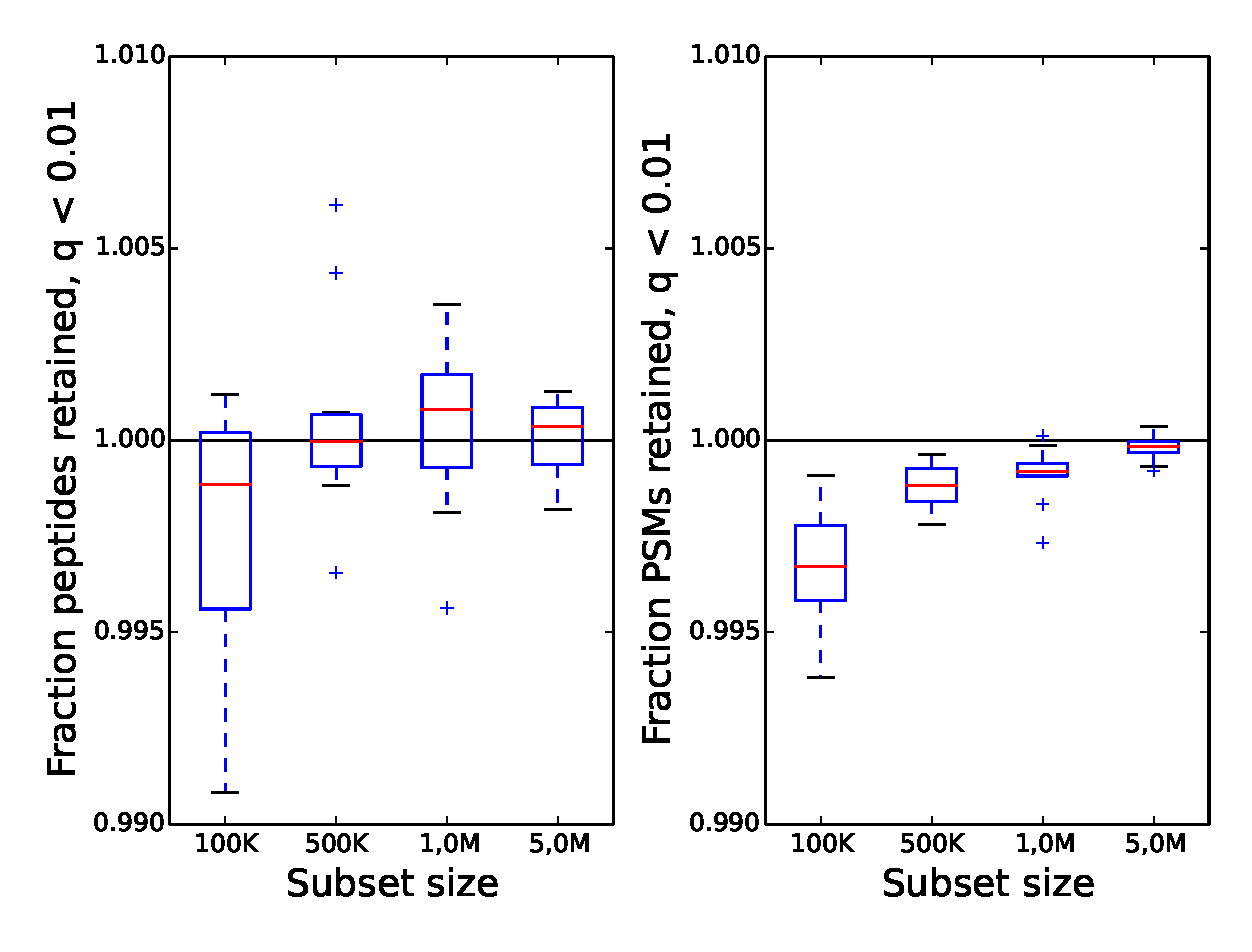
\includegraphics[width=0.6\linewidth]{./img/subset-performance}
\caption{\label{fig:subset}\textbf{Using subsets of the $73$ million
target+decoy PSMs for SVM training retains the number of significant
PSMs and peptides as training using the full set.} We evaluated subset
sizes of $100\,000, 500\,000, 1\,000\,000$ and $5\,000\,000$ PSMs to
train the SVMs, repeating this for $10$ randomized sets, and scored
all $73$ million PSMs using the resulting support vectors. We plotted
the ratio of significant PSMs and peptides at a $q$ value threshold of
$0.01$ as the fraction compared to using the full training set of $73$
million PSMs. The number of significant PSMs and unique peptides does
not drop significantly for even subsets of $100\,000$ PSMs.}
\end{center}
\end{figure}

To assess the accuracy of protein inference methods, we analyzed the
{\em hm\_yeast} set and compared the $q$ values reported based on the
decoy model, $FDR_{REV}$, to the fraction of entrapment proteins in
the set of identified target proteins, which we will call ``Observed
$FDR_{TRAP}$''. Technically, there is a discrepancy in underlying null
hypothesis of these two entities. The $FDR_{REV}$ has the null
hypothesis that the protein's peptide identifications came from
incorrect PSMs, while the Observed $FDR_{TRAP}$ employs the null
hypothesis that the protein is absent from the sample~\cite{the:how}.
As a counter measure, we strived to mitigate the problem by ensuring
that the entrapment database is very large compared to the sample
database, and thereby reducing the frequency of inadvertently
identifed absent sample proteins.

%FIXME: find a better reference for protein grouping approach?
First, we compared the four protein inference methods while retaining
the shared peptides. We grouped proteins that had the same set of
identified peptides, and also added proteins whose identified peptides
formed a strict subset of this set to such a
group~\cite{serang2012review}. To reduce the effect of proteins
breaking away from the group due to low-scoring, incorrect peptide
identifications that are unique to that protein, a peptide-level FDR
threshold was set at $10\%$. The decoy models based on the reversed
protein database systematically produced anti-conservative estimates
(Figure \ref{fig:shared-accuracy}).

Fisher's method and the product of peptide-level PEPs manage to
provide reasonable estimates from about $5\%$ protein-level FDR. For
the two-peptide rule, not enough decoy proteins remain to see if the
FDR estimates will become more accurate at some point, whereas the
best scoring peptide approach never manages to recover. Taking
stricter peptide-level thresholds generally improved the accuracy at
the cost of larger protein groups and, in the case of the two-peptide
rule, reduced sensitivity. However, going down to $5\%$ or even $1\%$
peptide-level FDR still produced anti-conservative protein-level FDR
estimates in the region below $1\%$ protein-level FDR.
%FIXME: add figure for this last claim?

\begin{figure}[!htp]
\begin{center}
\begin{tabular}{cc} 
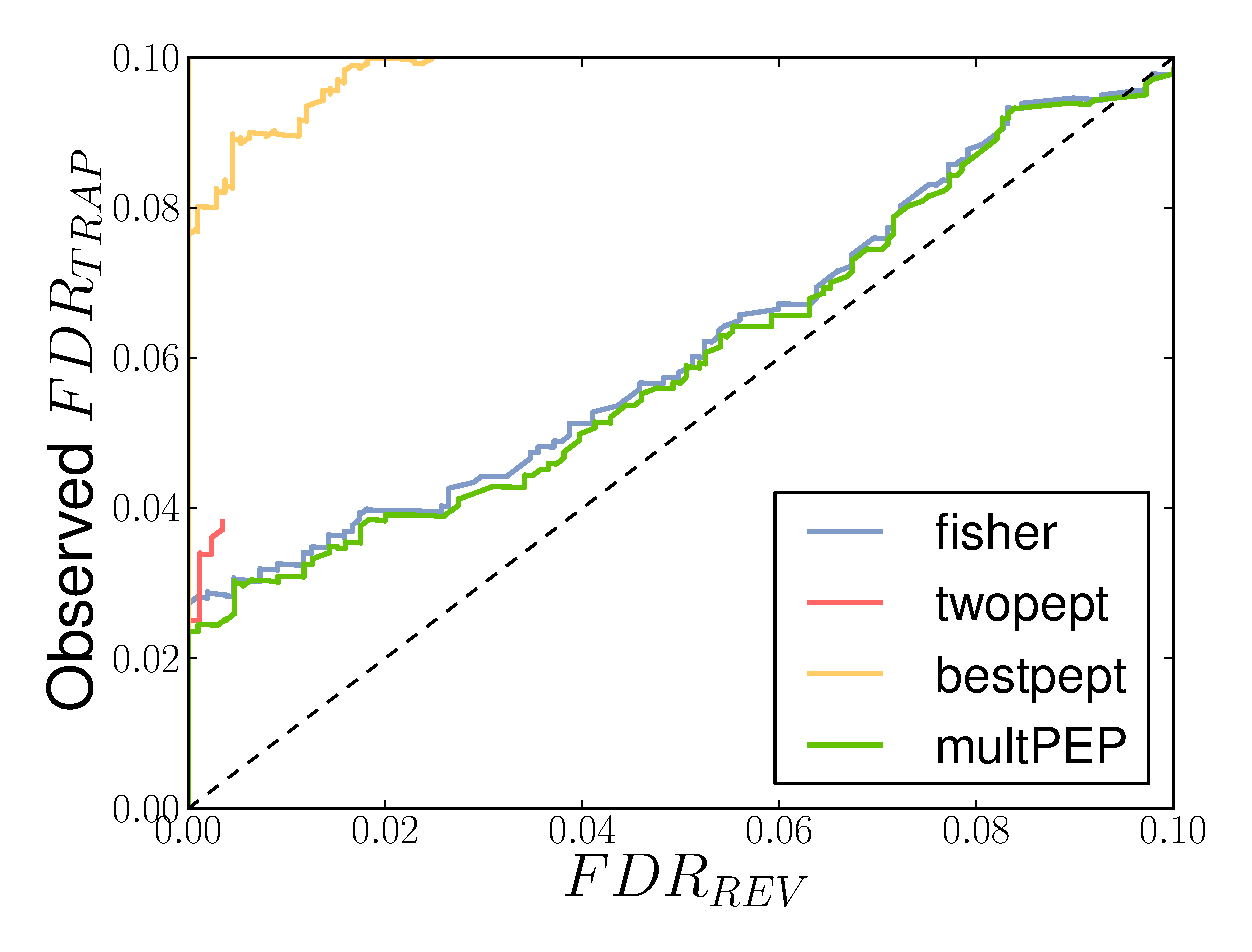
\includegraphics[width=0.45\linewidth]{./img/shared-pept-accuracy} &
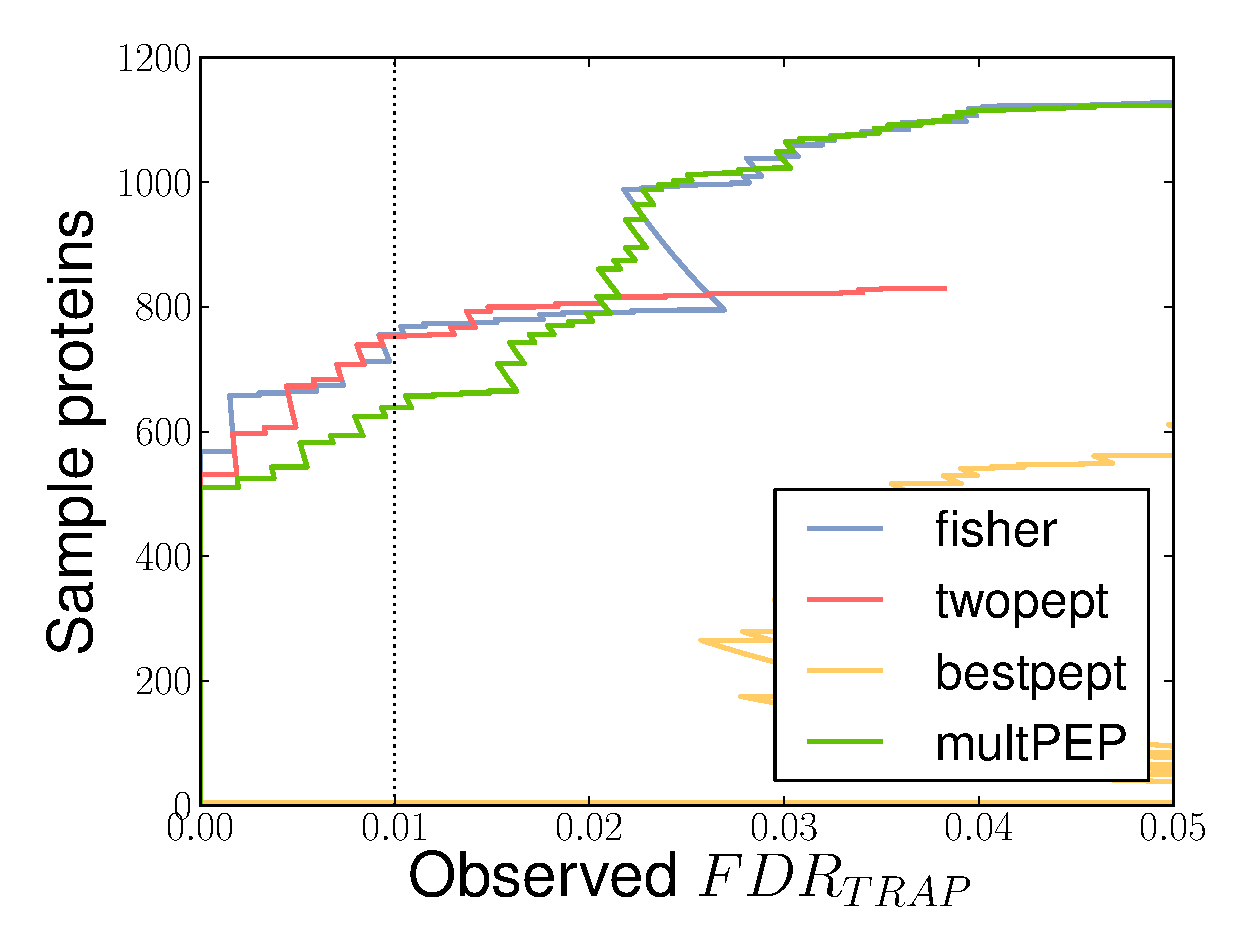
\includegraphics[width=0.45\linewidth]{./img/shared-pept-performance}
\\
(A) & (B)
\end{tabular}

\caption{\label{fig:shared-accuracy}\textbf{Retaining shared peptides
breaks the calibration of the decoy model for all protein inference
methods.} (A) We plotted the reported $q$ values from the decoy model,
$FDR_{REV}$, against the fraction of entrapment proteins in the set of
identified target proteins, ``Observed $FDR_{TRAP}$''. All four
methods produce anti-conservative FDR estimates. Fisher's method and
the product of peptide-level PEPs recover from around $5\%$
protein-level FDR, but the two peptide rule and best scoring peptide
approach do not seem to recover. (B) We plotted the number of sample
proteins, which can be considered an estimate for the number of true
identifications, against the ``Observed $FDR_{TRAP}$''. Whereas
Fisher's method, the product of peptide-level PEPs and the two peptide
rule initially pick up many sample proteins, the best scoring peptide
approach immediately breaks down.}
\end{center} 
\end{figure}

Second, we considered an approach using only peptides that are unique
to a single protein. However, this could cause some proteins to become
unidentifiable if there set of peptides was equal to that of another
protein or formed a subset of it. Therefore, we used the approach to
handling shared peptides from Nesvizhskii {\em et
al.}~\cite{nesvizhskii2003statistical}. Here, proteins are grouped
that are indistinguishable based on their theoretical proteolytically
digested peptides, rather than their experimentally discovered
peptides. We retain the peptides that are unique to such a protein
group, rather than to a single protein. Especially for databases
containing many proteoforms for a gene, this can considerably increase
the number of protein entities, {\em i.e.}, single proteins or protein
groups, with a peptide uniquely identifying it (Table
\ref{tab:duplicate-proteins}).

\begin{table}[!htp]
  \begin{center}
  
\begin{tabular}{|l|r|r|r|}
\hline
Human protein DBs & Swissprot & Swissprot+TrEMBL & Ensembl\\
\hline
Number of protein sequences & 20\,201 & 69\,714 & 101\,933\\
\hline
%\#unique peptide sequences & 586\,424 & 664\,801 & 672\,519\\
%\hline
Number of proteins with protein-specific peptide(s) & 19\,938 & 52\,834 &
49\,871\\
\hline
Number of protein groups & 20\,104 & 58\,605 & 68\,370\\
\hline
Number of protein groups with protein group-specific peptide(s) & 19\,978 &
54\,292 & 58\,929\\
\hline
\end{tabular}

  \end{center}
  \caption{\label{tab:duplicate-proteins}\textbf{The protein grouping
approach of Nesvizhskii {\em et al.} can increase the number of
identifiable protein entities considerably.} We did a fully tryptic
digestion with no miscleavages of three human protein databases:
Swissprot, Swissprot together with TrEMBL and Ensembl. We considered
peptides with lengths of $6$ to $50$ amino acids. TrEMBL and Ensembl
contain many proteoforms and therefore benefit signficantly from this
particular protein grouping approach in terms of number of
identifiable protein entities, {\em i.e.}, single proteins or protein
groups. Note that, unfortunately, some protein groups will remain
unidentifiable, because all their peptides are shared with at least
two different protein groups.}
\end{table}

Using this more conservative approach, all four methods now gave
accurate protein-level FDR estimates and a comparable number of
protein identifications as the approach with shared peptides retained
(Figure \ref{fig:unique-accuracy}). The two peptide rule was the only
method clearly performing worse than the others in terms of
identified protein groups.

\begin{figure}[!htp]
\begin{center}
\begin{tabular}{cc} 
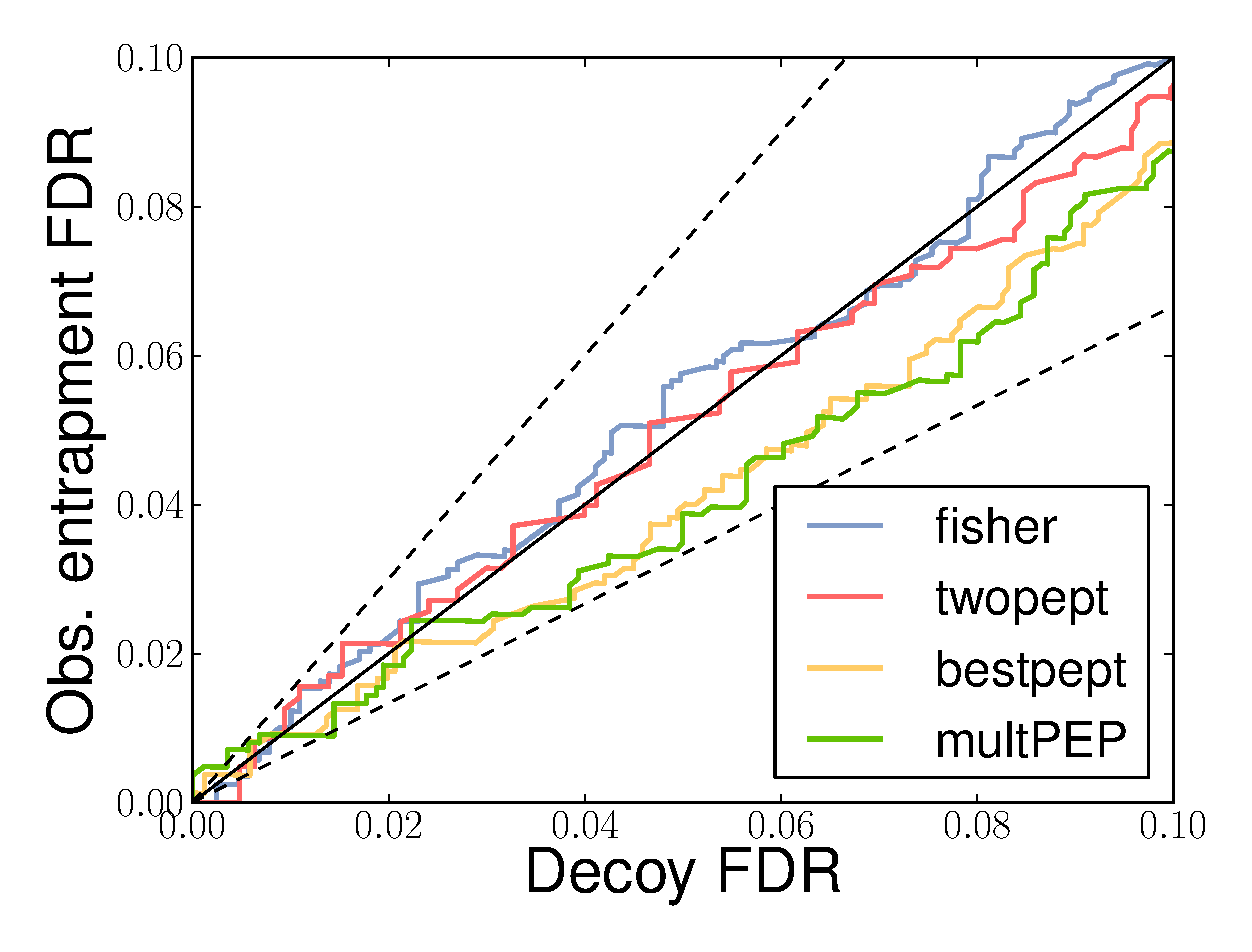
\includegraphics[width=0.45\linewidth]{./img/unique-pept-accuracy} &
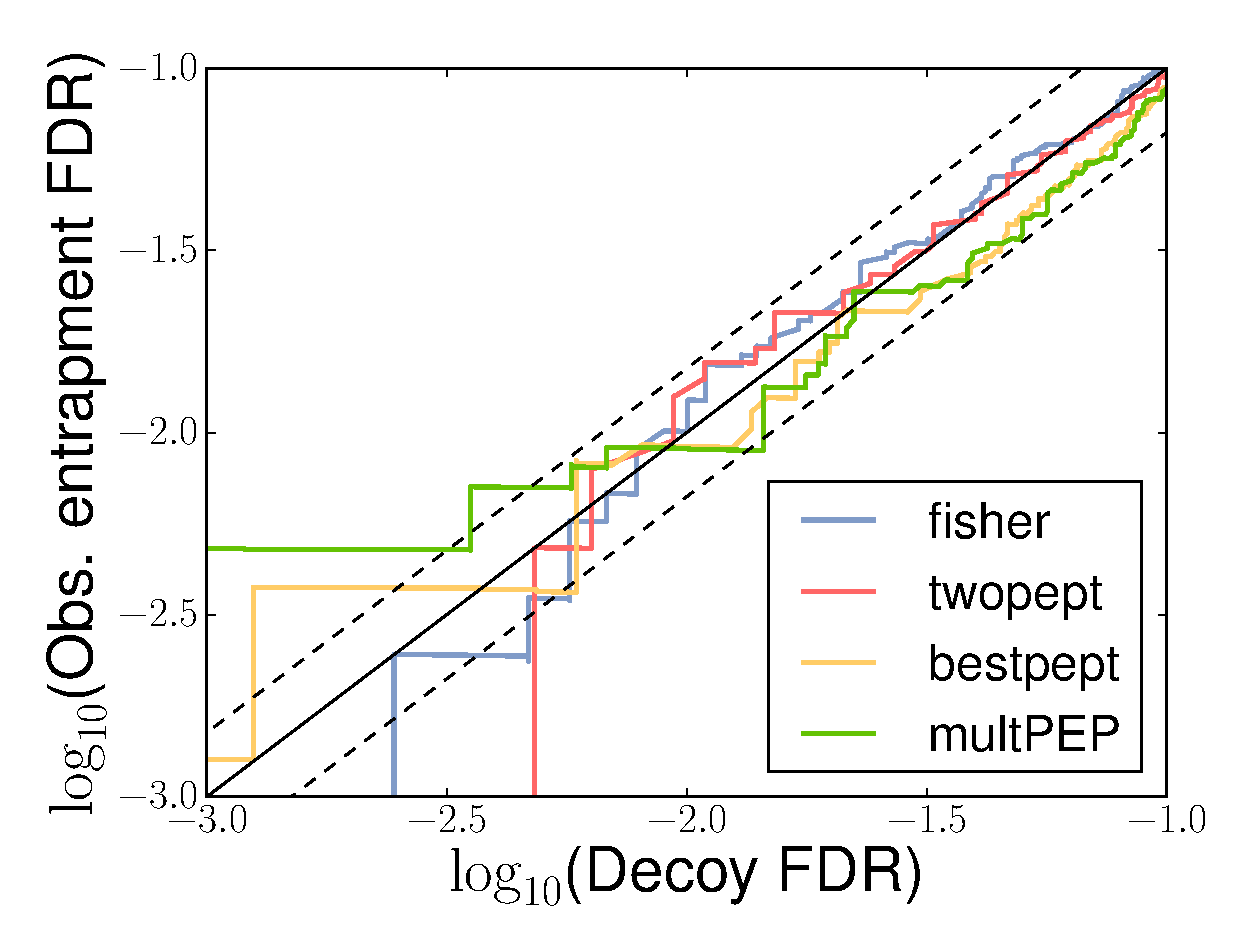
\includegraphics[width=0.45\linewidth]{./img/unique-pept-accuracy-log}
\\
(A) & (B)
\end{tabular}
\begin{tabular}{c}
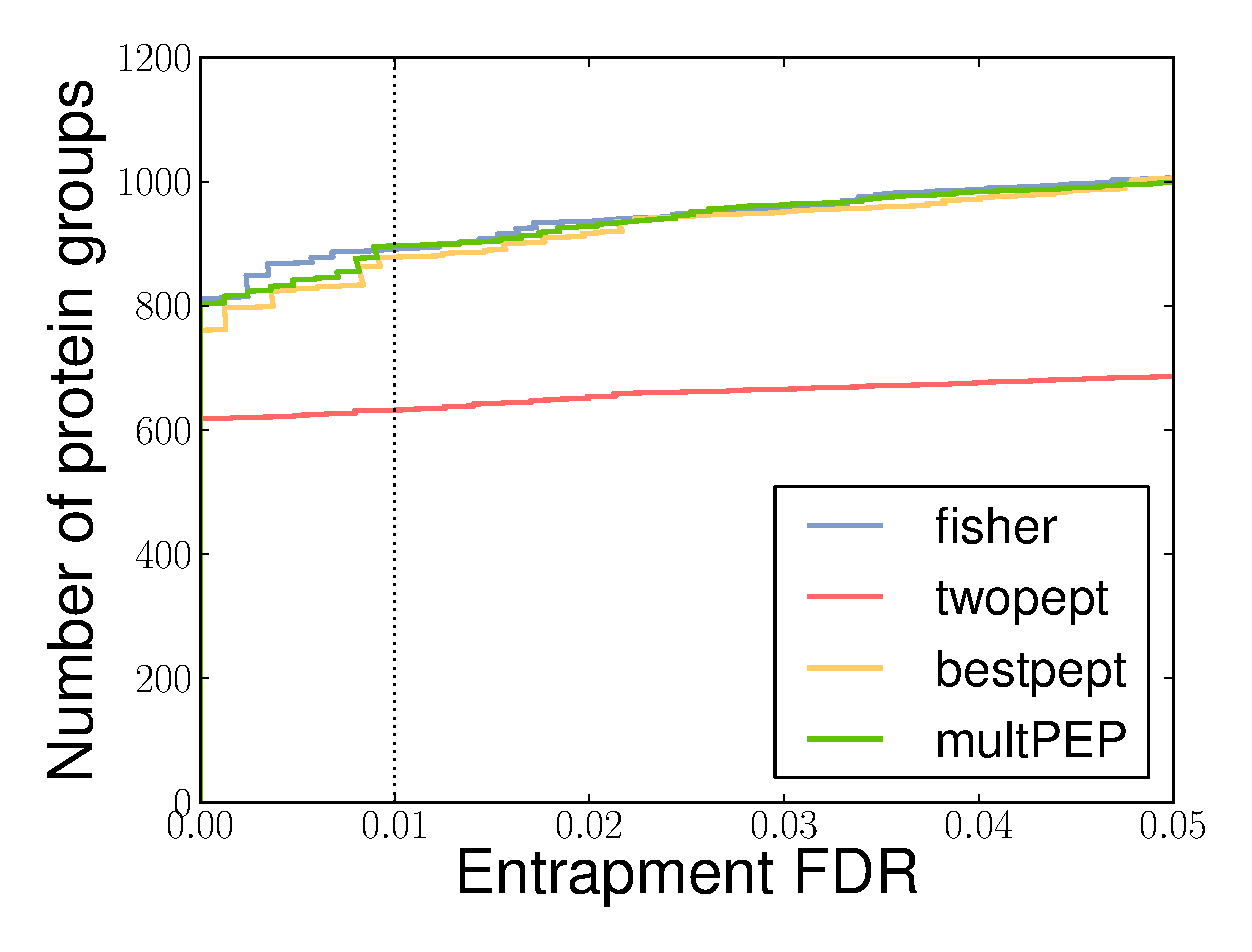
\includegraphics[width=0.45\linewidth]{./img/unique-pept-performance}
\\
(C)
\end{tabular}
\caption{\label{fig:unique-accuracy}\textbf{Using only protein-unique
peptides gives accurate estimates of the false discovery rate.} (A) We
plotted $FDR_{REV}$ against ``Observed $FDR_{TRAP}$'' as in Figure
\ref{fig:shared-accuracy}A. All four methods produce
accurate FDR estimates. The multiplication of peptide-level PEPs and
the best scoring peptide approach are slightly more conservative than
the other two methods. (B) We made a logarithmic plot of the region
$[0.001, 0.1]$ with the same axes as in (A). This showed that the
protein-level FDR estimates work reasonably well in this low region,
but break down somewhere in the $[0.001, 0.01]$ range, due to the low
density of decoy proteins in that region. (C) We plotted the number of
sample proteins against the ``Observed $FDR_{TRAP}$'' as in Figure
\ref{fig:shared-accuracy}B. Fisher's method, the product of
peptide-level PEPs and the best scoring peptide approach all perform
about equally, while the two peptide rule is much less sensitive.}
\end{center}
\end{figure}

From these results, it became clear that taking only unique peptides
together with the protein grouping approach from Nesvizhskii {\em et
al.} would be the most robust choice, regardless of the protein
inference method. To assess the performance using this strategy on
large-scale data, we applied the four methods on the {\em Kim} set.
Even for such large-scale data, all four protein inference methods
take less than a minute processing time due to their simplicity. We
looked at the number of identified proteins at $1\%$ reported
protein-level FDR (Table~\ref{tab:pandey-stats}). From these results
we concluded, in agreement with Savitski {\em et al.}, that the best
scoring peptide approach was indeed the superior alternative and
implemented this protein inference method in the latest Percolator
package. 

\begin{table}[!htp]
  \begin{center}
    \begin{tabular}{|l|r|r|}
    \hline
    partial digestion & Swissprot & Swissprot+TrEMBL\\
    \hline
    Best scoring peptide & 12\,370 & 5\,909\\
    \hline
    Product peptide-level PEPs & 11\,968 & 5\,626\\
    \hline
    Two peptide rule & 11\,409 & 4\,231\\
    \hline
    Fisher's method & 8\,964 & 3\,717\\
    \hline
    \end{tabular}
  \end{center}
  \caption{\label{tab:pandey-stats}\textbf{Using the best scoring
peptide as a protein's representantive identified the most protein
groups.} We examined the number of protein identifications for the
four protein inference method using only peptides unique to one of
the protein groups formed by the approach from Nesvizhskii {\em et
al.}. The best scoring peptide approach identified the most protein
groups with a $3\%$ margin over the second best method. Fisher's
method identified much fewer proteins than the other three methods,
due to incorrect peptides dragging down the $p$ value of correct
proteins. The many proteoforms in the TrEMBL database caused a large
drop in the number of identifications for all methods.}
\end{table}

\section*{Discussion}

We demonstrated that Percolator 3.0 can calculate protein-level FDRs
on a human proteome scale study, in this case $73$ million PSMs, in a
matter of minutes on a commodity computer.

The subset scoring shows great stability even when only sampling a
tiny fraction, as small as $0.1\%$, of the original number of PSMs.
The {\em Kim} set might not be as representative for other types of
studies that have greater heterogeneity, but it seems likely that the
idea will hold as long as the subsets are not chosen too small.
Particularly our subset sampling strategy, that trains and tests on
the same data will only avoid problems of overfitting when the
strategy is carried out on large datasets.

The most succesful protein inference method turned out to be the one
where proteins were grouped by their theoretical peptide sets and only
the best scoring peptide was considered. This implies that the
algorithm excludes the majority of the PSMs in its final protein list,
something that may feel quite unsatisfying. With regards to the
discarded shared peptides, large-scale studies give us the luxury of a
deep coverage of the present peptides and therefore identify many
peptides that are unique to a protein. This mitigates the problem of
ignoring shared peptides in terms of number of protein identifications
and makes the task of protein inference much simpler and intuitive.

The main problem in including the evidence of the other lower scoring
peptide identifications is the difficulty in dealing with incorrect
peptide identifications belonging to correct protein identifications.
This can clearly be seen in the poor performance of Fisher's method
for combining $p$ values on the {\em Kim} set. Setting
peptide-level thresholds can actually bring Fisher's method up to par
with the best scoring peptide approach (data not shown). However,
it does not produce signficantly more protein identifications,
while introducing an extra parameter that needs to be set correctly.

The protein grouping of Nesvizhskii {\em et al.} employed here still
suffers from the problem that an identification of a protein group
leaves open the question which proteins in the group are actually
correct. Here, we interpreted it using the null hypothesis that all
proteins in the group are incorrect, {\em i.e.}, an identified protein
group means that we expect at least one of the proteins to be correct,
but we are agnostic about which one. Compared to the conventional
protein grouping approach, however, the groups are much smaller and
this unsatisfactory answer does not have to be given as often.
Furthermore, if genes, rather than proteoforms are the entities of
interest, using databases with few proteoforms such as Swissprot
should do the job.

We realize that other parts of the shotgun proteomics analysis
pipeline might still have significantly higher computing requirements
than Percolator, but fortunately these can often readily be
parallelized as the runs can be analyzed independently. However,
obtaining significance measures per run or data set and combining them
afterwards is not at all straightforward and should be handled with
the greatest caution~\cite{serang2015solution}. This new version of
Percolator opens up for the possibility of easily obtaining
statistical signficance measures on aggregated data from a great
number of runs without running this risk.

\section*{Acknowledgements}

%FIXME: add acknowledgement to Uppmax? LK: Check standard formulation
% from SNIC

\bibliography{percolator}{} 
\bibliographystyle{plain}

\end{document}
